% Created 2020-09-05 Sat 19:13
% Intended LaTeX compiler: lualatex
\documentclass[11pt]{article}
\usepackage{graphicx}
\usepackage{grffile}
\usepackage{longtable}
\usepackage{wrapfig}
\usepackage{rotating}
\usepackage[normalem]{ulem}
\usepackage{amsmath}
\usepackage{textcomp}
\usepackage{amssymb}
\usepackage{capt-of}
\usepackage{hyperref}
\usepackage{tabularx}
\usepackage{etoolbox}
\makeatletter
\def\dontdofcolorbox{\renewcommand\fcolorbox[4][]{##4}}
\AtBeginEnvironment{minted}{\dontdofcolorbox}
\makeatother
\usepackage[newfloat]{minted}
\usepackage{amsthm}
\theoremstyle{definition}
\newtheorem{definition}{Definition}[section]
\usepackage{unicode-math}
\usepackage{unicode}
\author{Mark Armstrong}
\date{Fall 2020}
\title{Introduction and overview\\\medskip
\large Principles of Programming Languages}
\hypersetup{
   pdfauthor={Mark Armstrong},
   pdftitle={Introduction and overview},
   pdfkeywords={},
   pdfsubject={An introduction and a brief overview of topics we will discuss in the course.},
   pdfcreator={Emacs 27.0.90 (Org mode 9.3.7)},
   pdflang={English},
   colorlinks,
   linkcolor=blue,
   citecolor=blue,
   urlcolor=blue
   }
\begin{document}

\maketitle

\section{Preamble}
\label{sec:org32b6f5f}
The preamble section of each notes will include
\begin{itemize}
\item notable references,
\begin{itemize}
\item i.e., specific chapters of our recommended/additional texts
from which the notes are derived, or which expand on the notes,
\end{itemize}
\item a table of contents, and
\item an update history, chronicling any major changes.
\begin{itemize}
\item Note the git commit history will provide a more fine-grained
record of upates.
\end{itemize}
\end{itemize}

\subsection{{\bfseries\sffamily TODO} Notable references}
\label{sec:org583a82b}
:TODO:

\subsection{{\bfseries\sffamily TODO} Table of contents}
\label{sec:orgc96bb03}
\begin{scriptsize}
\begin{itemize}
\item \hyperref[sec:org32b6f5f]{Preamble}
\end{itemize}
\end{scriptsize}

\section{Introduction}
\label{sec:orge59eff7}
This section of notes introduces the course and the staff,
and lays out a few central concepts.

\section{Welcome}
\label{sec:org4eab0a7}
\begin{center}
Welcome to the course!
\end{center}

\subsection{Instructor: Mark Armstrong}
\label{sec:orgc2ed85e}
\begin{quote}
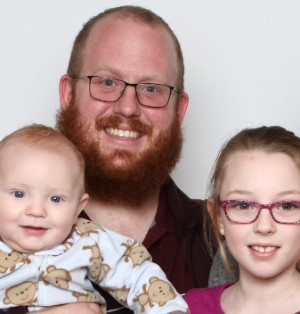
\includegraphics[width=200px]{./media/markarmstrong.jpg}
\end{quote}

\begin{itemize}
\item Email: \url{mailto:armstmp@mcmaster.ca}
\item Website: \url{https://armkeh.github.io}
\end{itemize}

\subsection{Teaching assistants}
\label{sec:org4cb5b42}
:TODO:

\section{Purpose and goals of this course}
\label{sec:org180a47b}
\subsection{Calendar description}
\label{sec:orgd3e33b0}
Design space of programming languages;
abstraction and modularization concepts and mechanisms;
programming in non-procedural (functional and logic) paradigms;
introduction to programming language semantics.

\subsection{Informal objectives}
\label{sec:orgfa83981}
\begin{itemize}
\item Investigate several programming languages.
\begin{itemize}
\item A relatively shallow but comprehensive survey.
\item Focusing on general-purpose languages.
\end{itemize}
\item \emph{Formally} describe programming language syntax and semantics.
\begin{itemize}
\item An application of theory learned previously.
\end{itemize}
\item Learn informal criteria by which to judge languages.
\begin{itemize}
\item Identify what languages fit what tasks.
\end{itemize}
\item Examine the origins of certain languages/groups of languages.
\begin{itemize}
\item Historical context provides insight into why languages
are designed the way they are.
\end{itemize}
\end{itemize}

\subsection{Course preconditions}
\label{sec:org99995fc}
Before beginning this course:

\begin{enumerate}
\item Students should know and understand:
\begin{enumerate}
\item Basic concepts about integers, sets, functions, \& relations.
\item Induction and recursion.
\item First order logic, axiomatic theories \& simple proof techniques.
\item Regular expressions \& context-free grammars.
\item Programming in imperative language
\item Basic concepts of functional programming languages.
\end{enumerate}
\item Students should be able to:
\begin{enumerate}
\item Produce proofs involving quantifiers and/or induction.
\item Understand the meaning of a given axiomatic theory.
\item Construct regular sets \& context-free languages.
\item Produce small to medium scale programs in imperative languages.
\item Produce small scale programs in functional languages.
\end{enumerate}
\end{enumerate}

\subsection{Course postconditions}
\label{sec:org67e1e33}
After completion of this course:

\begin{enumerate}
\item Students should know and understand:
\begin{enumerate}
\item The basics of several programming languages.
\item Formal definitions of syntax \& semantics for various
simple programming languages.
\item Various abstraction \& modularisation techniques
employed in programming languages.
\end{enumerate}
\item Students should be able to:
\begin{enumerate}
\item Reason about the design space of programming languages,
in particular tradeoffs \& design issues.
\item Produce formal descriptions of syntax \& semantics
from informal descriptions, identifying ambiguities.
\item Select appropriate abstraction \& modularisation techniques
for a given problem.
\item Produce (relatively simple) programs in various languages,
including languages from non-procedural paradigms.
\end{enumerate}
\end{enumerate}

\subsection{{\bfseries\sffamily TODO} Formal rubric for the course}
\label{sec:org35f090c}
This was last year's rubric. It needs tweaking.

\begin{scriptsize}
\begin{center}
\begin{tabular}{|l|l|l|l|l|}
\hline
Topic & Below & Marginal & Meets & Exceeds \\
\hline
Familiarity & Shows some & Shows & Achieves & Achieves \\
with various & competence & competence & competence & competence \\
programming & in & in & with the & with \\
languages & procedural & procedural & basic & intermediate \\
(PLs) & languages, & languages & usage of & usage of \\
 & but not & and limited & various & various \\
 & languages & competence & languages & languages \\
 & from other & in & & \\
 & paradigms & languages & & \\
 & & from other & & \\
 & & paradigms & & \\
\hline
Ability to & Cannot & Identifies & Identifies & Identifies \\
identify and & consistently & such & such & sucj \\
make use of & identify & constructs, & constructs & constructs \\
abstraction, & such & but does not & and shows & and shows \\
modularisation & constructs & consistently & some ability & mastery of \\
constructs & & make use of & to make use & them when \\
 & & them when & of them when & programming \\
 & & programming & programming & \\
\hline
Ability to & Unable or & Comprehends & Makes only & Consistently \\
comprehend and & rarely & given & minor & fully \\
produce formal & able to & grammars, & errors & understands \\
descriptions & comprehend & but & regarding & given \\
of PL syntax & given & produces & precedence & grammars and \\
 & grammars; & grammars & or & produces \\
 & does not & which are & ambiguity & correct \\
 & identify & ambiguous & when & grammars. \\
 & ambiguity & or which do & reading or & \\
 & or & not & producing & \\
 & precedence & correctly & grammars & \\
 & rules & specify & & \\
 & & precedence & & \\
\hline
Ability to & Rarely or & Usually & Comprehends & Comprehends \\
comprehend and & never & comprehends & such & such \\
produce & comprehends & such semantic & semantic & semantic \\
operational & such & descriptions, & descriptions & descriptions \\
semantics for & semantic & but cannot & and produces & and produces \\
simple PLs & descriptions & consistently & them with & them without \\
 & & produce them & only minor & errors \\
 & & & errors & \\
\hline
Ability to & Rarely or & Inconsistently & Consistently & Consistently \\
comprehend & never & comprehends & comprehends & comprehends \\
denotational & comprehends & such semantic & such & and can \\
and axiomatic & such & descriptions & semantic & produce some \\
semantics for & semantic & & descriptions & simple \\
simple PLs & descriptions & & & semantic \\
 & & & & descriptions \\
\hline
\end{tabular}
\end{center}
\end{scriptsize}

\section{{\bfseries\sffamily TODO} “Principles of programming languages”}
\label{sec:orgf4f9590}
\section{{\bfseries\sffamily TODO} Abstraction}
\label{sec:orge9a1c9d}
\section{{\bfseries\sffamily TODO} Exercises}
\label{sec:org149b6a4}
\end{document}
